\chapter{Related work}

\section{DeeperCut\mbox{:} A Deeper, Stronger, and Faster Multi-Person Pose Estimation Model \cite{DBLP:journals/corr/InsafutdinovPAA16}}

\subsection{Problem}
The goal of this paper is to advance the state-of-the-art of articulated pose estimation in scenes with multiple people.

\subsection{Methods}
\par Part Affinity Fields (PAFs), to learn to associate body parts with individuals in the image. The architecture encodes global context, allowing a greedy bottom-up parsing step that maintains high accuracy while achieving realtime performance.	
\par The part affinity is a 2D vector field for each limb: for each pixel in the area belonging to a particular limb, a 2D vector encodes the direction that points from one part of the limb to the other. Each type of limb has a corresponding affinity field joining its two associated body parts.


\subsection{Data}
\par The MPII human multi-person dataset \cite{database2dhuman}  and the COCO 2016 keypoints challenge dataset \cite{coco2016}. These two datasets collect images in diverse scenarios that contain many real-world challenges such as crowding, scale variation, occlusion, and contact.
\par MPII Human Pose dataset is a state of the art benchmark for evaluation of articulated human pose estimation. The dataset includes around 25K images containing over 40K people with annotated body joints. The images were systematically collected using an established taxonomy of everyday human activities.


\subsection{Performance and comparisons}
Evaluation is done on two single-person and two multi-person pose estimation benchmarks. The proposed approach significantly outperforms best known multi-person pose estimation results while demonstrating competitive performance on the task of single person pose estimation.

\section{Human Pose Estimation from Monocular Images: A Comprehensive Survey
\cite{humanmonocular}}

\subsection{Problem}
\par In this paper, a comprehensive survey of human pose estimation from monocular images is carried out including milestone works and recent advancements. The goal of our application is to provide initialization for automatic video surveillance. 
\subsection{Methods}
\par Based on one standard pipeline for the solution of computer vision problems, this survey splits the problem into several modules: feature extraction and description, human body models, and modeling methods. There are additional sections for motion-related methods in all modules: motion features, motion models, and motion-based methods.

\subsection{Data}
The paper collects 26 publicly available datasets for validation and provides error measurement methods that are frequently used.
\subsection{Performance and comparisons}
\par The first survey that includes recent advancements on human pose estimation based on deep learning algorithms. Although deep learning algorithms bring huge success to many computer vision problems, there are no human pose estimation reviews that discuss these works. In this survey, about 20 papers of this category are included. This is not a very large number compared to other problems, but this is a inclusive survey considering the relatively few works addressing this problem.

\section{PersonLab: Person Pose Estimation and Instance Segmentation with a Bottom-Up, Part-Based, Geometric Embedding Model
\cite{DBLP:journals/corr/abs-1803-08225}}

\subsection{Problem}
\par Paper try to solve the task of 2-D pose estimation and instance segmentation of people in multi-person images using an efficient single-shot model based on a box-free bottom-up approach. 
The study contributes to computer vision applications such as smart photo editing, person and activity recognition, virtual or augmented reality, and robotics. 

\subsection{Methods}
 Bottom-up approach for pose estimation and segmentation:
 \begin{itemize}
 \item localizing identity-free semantic entities (individual keypoint proposals or semantic person segmentation labels, respectively)
    \item grouping them into person instances:
    \begin{itemize}
        \item use a greedy decoding process to group them into instances
        \item train network to predict instance-agnostic semantic person segmentation maps
        \item for every person pixel we also predict a set vectors to each of the K keypoints of the corresponding person instance. (corresponding vectors fields can be thought as a geometric embedding representation and induce basins of attraction around each person instance, leading to an efficient association algorithm)
         \begin{itemize}
         \item For each pixel $x_i$, they predict the locations of all K keypoints for the corresponding person that $x_i$ belongs to
         \item then compare this to all candidate detected people j (in terms of average keypoint distance), weighted by the keypoint detection probability 
         \item if this distance is low enough, we assign pixel i to person j

         \end{itemize}
    \end{itemize}
 \end{itemize}


\subsection{Data}
Standard COCO keypoint dataset \cite{coco2016}.

\subsection{Performance and comparisons}
\begin{itemize}
    \item compared to the best previous bottom-up approach they improve keypoint AP (Average Precision) from 0.655 to 0.687
    \item compared to the strong top-down FCIS method \cite{DBLP:journals/corr/LiQDJW16} improve mask AP from 0.417 to 0.386
\end{itemize}


\section{Towards Accurate Multi-person Pose Estimation in the Wild
\cite{DBLP:journals/corr/PapandreouZKTTB17}}

\subsection{Problem}
\par Paper try to solve the task of multi-person detection and 2D pose estimation based on a top-down approach (2-D localization of human joints on the arms, legs, and keypoints on torso and the face).
The study want to localize people, understand the activities they are involved in, understand how people move for the purpose of Virtual/Augmented Reality, and learn from them to teach autonomous systems.


\subsection{Methods}
 Top-down approach consisting of two stages:
 \begin{itemize}
    \item first stage, predict the location and scale of boxes which are likely to contain people, use Faster RCNN detector.
    \item second stage, estimate the keypoints of the person potentially contained in each proposed bounding box:
        \begin{itemize}
            \item for each keypoint type predict dense heatmaps and offsets using a fully convolutional ResNet
            \item combine these outputs by a novel aggregation procedure to obtain highly localized keypoint predictions

             \begin{itemize}
             \item use keypoint-based Non-Maximum-Suppression (NMS), instead of the cruder boxlevel NMS
             \item keypoint-based confidence score estimation, instead of box-level scoring
    
             \end{itemize}
        \end{itemize}
 \end{itemize}


\subsection{Data}

Training data: standard COCO keypoint dataset \cite{coco2016}, which annotates multiple people with 12 body and 5 facial keypoints.


\subsection{Performance and comparisons}
\begin{itemize}
    \item average precision of 0.649 on the COCO test-dev set and the 0.643 test-standard sets, outperforming the winner of the 2016 COCO keypoints challenge and other recent state-of-art.
    \item using additional in-house labeled data we obtain an even higher average precision of 0.685 on the test-dev set and 0.673 on the test-standard set, more than 5\% absolute improvement compared to the previous best performing method on the same dataset.

\end{itemize}



\section{Realtime Multi-Person 2D Pose Estimation using Part Affinity Fields
\cite{DBLP:journals/corr/CaoSWS16}}

\subsection{Problem}
\par The purpose is to recognize a layout of the body parts, based on the pose estimation and Pose Affinity Fields (PAF).

\subsection{Methods}
 \begin{itemize}
    \item Part affinity fields(PAF): is a set of 2D vector fields that encode the location and orientation of the limbs. It is a set of vectors that encodes the direction from one part of the limb to the other; each limb is considered as an affinity field between body parts.
    \item Estimation of body-part confidence maps.
 \end{itemize}
\begin{figure}[htbp]
	\centerline{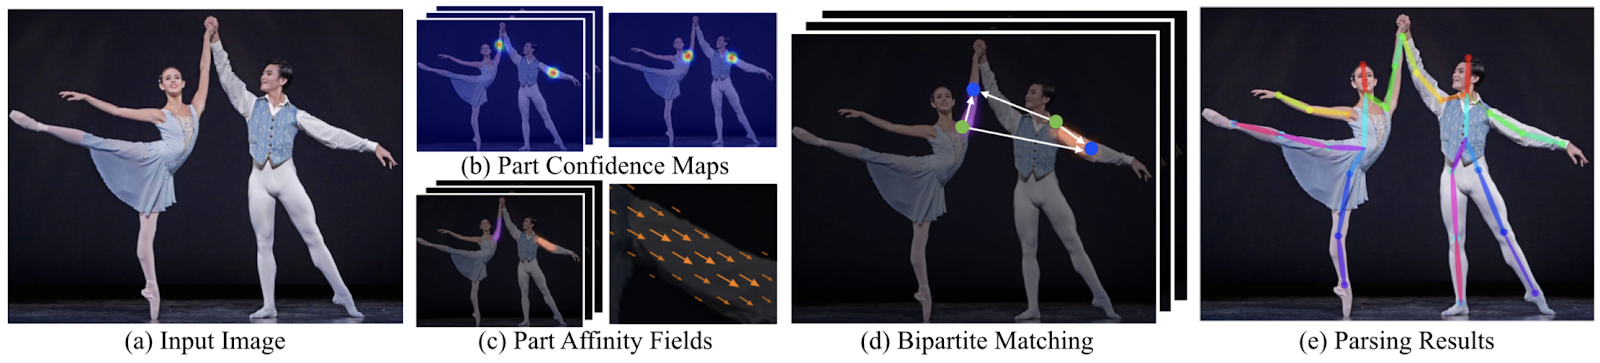
\includegraphics[scale=0.25]{fig/algoritm-ann.png}}  
	\caption{Overall pipeline \cite{DBLP:journals/corr/CaoSWS16}}
\end{figure}

\subsection{Data}
\par As an input we have an image. This method simultaneously infers two maps with body-parts, as you can see in b figure and runs a special bipartite matching algorithm. In the end it assemble the body parts into full body poses.
\par Training data: standard COCO keypoint dataset \cite{coco2016} and the MPII human multi-person
dataset \cite{database2dhuman}
